\documentclass[a4paper]{article}

\usepackage[french]{babel}
\usepackage[utf8]{inputenc}
\usepackage{graphicx}
\usepackage{pdfpages}

\title{Small World : Rapport de Modélisation \\ INSA de Rennes - 4INFO}

\author{Axel CARO, Maximilien RICHER}

\date{\today}

\begin{document}
\maketitle

\paragraph{}
Ce document présente les résultats de la phase de modélisation du projet de quatrième année proposé en enseignement de \textit{Programmation et Modélisation orientées objet}.

\newpage

\section*{Introduction}
\paragraph{}
Le projet proposé consiste en la réalisation d'un jeu vidéo tour par tour, basé sur le jeu de plateau \textit{SmallWorld}. Au cours d'une partie, les joueurs s'affrontent pendant un certain nombre de tours, afin prendre le contrôle d'un territoire. Ce projet met l'accent sur les différentes phases de la réalisation d'un projet d'application orientée objet. La modélisation, l'utilisation de patrons de conceptions, l'organisation du code, l'implémentation, l'utilisation de librairies dynamiques, l'interfaçage entre plusieurs langages, la gestion d'IHM et les phases de tests sont des points clés des objectifs pédagogiques de ce projet.

\section{Présentation des règles du jeu}

\subsection{But du jeu}
\paragraph{}
Le but de SmallWorld est d'accumuler des points de victoire.
À la fin de chaque tour de jeu, le joueur compte les points gagnés et les ajoute à son total. Au bout d'un nombre de tour défini au préalable, le jeu s'arrête et le joueur ayant le plus de point remporte la partie. Une partie peut également s'interrompre si un des joueurs élimine l'ensemble des unités de l'adversaire. Un joueur qui ne possède plus d'unités perd la partie, quel que soit son total de point.

\paragraph{}
\textbf{Déroulement d'une partie}
\begin{itemize}
    \item Choix de la configuration du plateau de jeu
    \item Choix des races
    \item Choix du joueur qui commence la partie
    \item Création du plateau de jeu
    \item Début du premier tour de jeu\\(\dots)
    \item Fin du dernier tour de jeu
    \item Décompte final des points
\end{itemize}

\subsubsection{Plateau de jeu}
\paragraph{}
Le jeu se déroule sur une plateau quadrillé de cases carrées dont la dimension dépend du nombre de joueurs et de la durée de la partie.\label{map_gen} Il est composé de cases de différents types : plaine, mer, montagne et forêt. La carte est généré de manière aléatoire, mais doit contenir le même nombre de case de chaque type.

\subsubsection{Unité}
\paragraph{}
Des unités sont placées sur le plateau, sur lequel elles peuvent être déplacées. Elles possèdent des points d'action, rechargé en début de tour, mais aussi une jauge de vie et des statistiques d'attaque et de défense.

\subsubsection{Races et décompte des points en fin de tour}
À la fin de chaque tour, le joueur compte les points gagné et les ajoutes à son total. Le montant des points gagné est déterminé en fonction de la race choisie et du type de terrain sur lequel ses unités sont placées.

\paragraph{}
\textbf{Configurations conseillées}
\begin{itemize}
    \item 2 joueurs, plateau de 6 par 6, 5 tours de jeu : 4 unités par joueur
    \item 2 joueurs, plateau de 10 par 10, 20 tours de jeu : 6 unités par joueur
    \item 2 joueurs, plateau de 14 par 14, 30 tours de jeu : 8 unités par joueur
\end{itemize}

\subsubsection{Préparation}
\paragraph{}
La préparation du jeu necéssite que le joueur choisisse le type de partie parmis les configurations proposées. 

\subsection{Déroulement d'un tour de jeu}
\paragraph{}
Chaque \textit{tour de jeu} est constitué de plusieurs \textit{tours de joueurs}. Ces tours sont séquentiels. Lors du premier tour de jeu, le joueur jouant le premier tour est tiré au hasard, et cet ordre est conservé durant le reste de la partie.

\paragraph{}
\textbf{Déroulement du tour}
\begin{itemize}
    \item Début du tour
    \item Déplacement des unités et combats
    \item Décompte des points
    \item Fin du tour
\end{itemize}

\subsection{Déplacement et combat}
\paragraph{}
Un joueur peut, durant son tour, déplacer une ou plusieurs unité lui appartenant. Une unité ne peut être déplacé que si il lui reste assez de point d'action pour effectuer le déplacement demandé. Le nombre de point d'action nécessaire dépend de la race du jouer et du type de la case de destination. Les déplacement ne peuvent s'effectuer que vers une case adjacente, et non en diagonale. Un déplacement vers une case occupée par un ou plusieurs alliées ets autorisé. Un déplacement vers une case occupée par une unité adverse engendre un combat.

\paragraph{}
Les combats sont détaillé plus bas\ref{fight_seq}. Il est possible d'attaquer une unité plusieurs fois de suite, à condition de disposer des points d'action nécéssaires.
\subsubsection{Combat au corps à corps}
Le combat au CaC est provoqué par un déplacement. Dans le cas de la mort de l'unité adverse, l'attaquant est déplacé sur sa case. Dans le cas contraire, il conserve sa position.
Il engendre une rispose de l'adversaire. Cette risposte n'influe pas sur les points d'action dont dispose celui-ci au tour suivant.
\subsubsection{Combat à distance}
Un combat à distance n'implique pas de déplacement. L'attaquant doit se trouver sur la même ligne ou la même colonne que sa cible, à deux cases de distance. Sur la case vide situé entre l'attaquant et sa cible peut se trouver une unité allié ou adverse sans que cela n'ai d'incidence sur le déroulement de l'attaque.
Ce combat se déroule sans contre-attaque de l'adversaire, et n'engendre aucun déplacement en cas de victoire. 
\section{Modélisation UML}
\paragraph{}
La phase de modélisation nous a conduit à réaliser plusieurs diagrammes UML, afin de représenter différents aspects de notre application. Nous présentons ci-après ces diagrammes, en explicitant leur contenu.

\subsection{Diagramme de paquetage}
\paragraph{}
Le diagramme suivant illustre la structuration à gros grain du code de notre application. On y retrouve les classes et interfaces que nous détaillerons dans la section \ref{DDC}.
Comme on peut le constater, nous n'avons pas hiérarchisé notre application selon plusieurs paquetages. En effet, les interactions entre nos classes et interfaces auraient conduit à des dépendances circulaires entre les éventuels paquetages, mais transformer le modèle afin d'éviter ces problèmes aurait résulté en une complexité des traitements beaucoup plus importante, ou en la création de trop nombreux paquetages.

\paragraph{}
Nous avons donc opté pour la simplicité de traitement. Les différentes classes et interfaces étant toutes liées, il nous semble inapproprié de les séparer dans des paquetages différents : les modifications éventuelles impacteront bon nombre d'entre elles, touchant à plusieurs des paquetages envisagés.

\paragraph{}
Par ailleurs, la séparation de notre application en paquetages "modèle" , "API" n'est pas pertinente, car ce projet ne porte que sur \textbf{une} implémentation du jeu proposé. Si plusieurs implémentations avaient été requises, la séparation précédente aurait alors eu du sens.

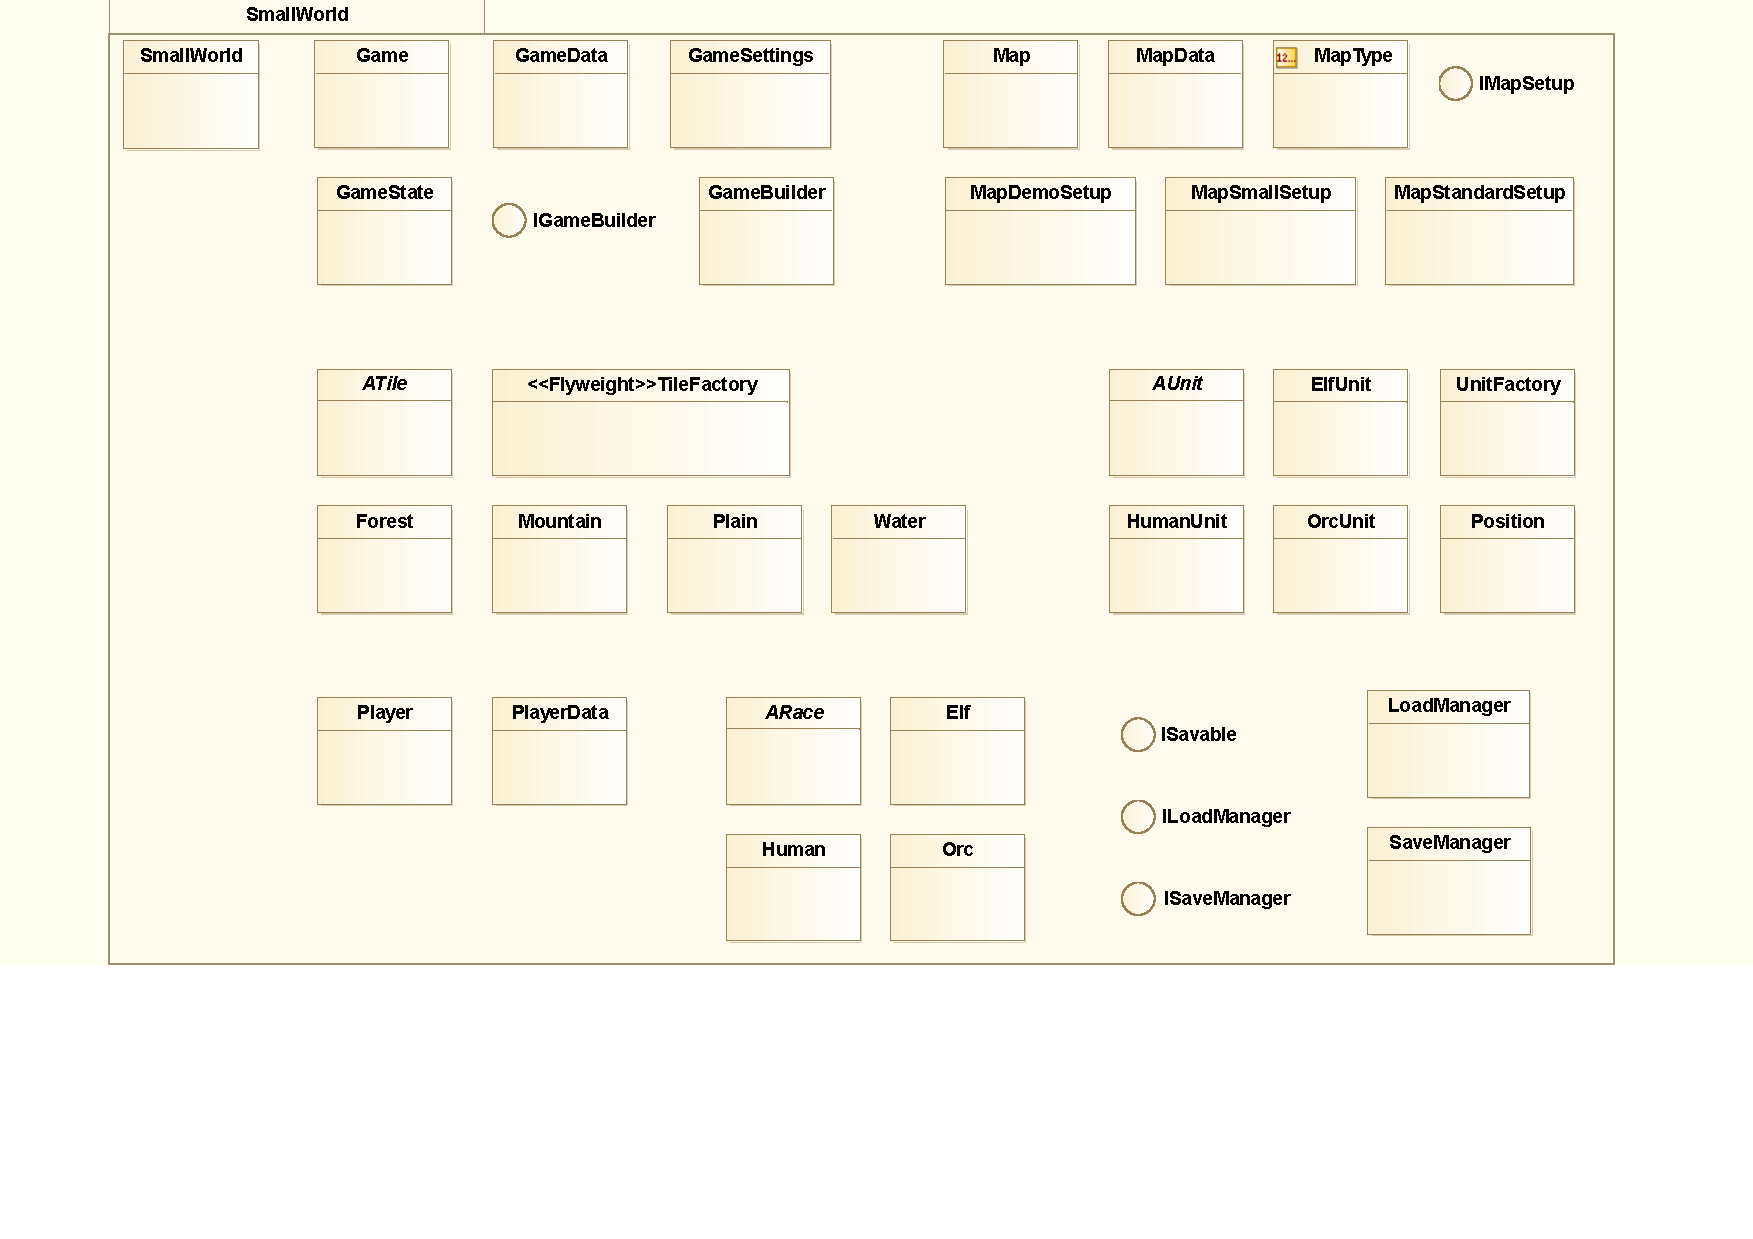
\includepdf[landscape=true]{images/packageDiagram.pdf}

\subsection{Diagramme de classes}
\label{DDC}
\paragraph{}
Le diagramme suivant illustre l'organisation en classes de notre application.
On distingue des regroupements de classes par thématiques : 
\begin{itemize}
    \item SmallWorld : la classe principale de l'application
    \item Game : gestion d'une partie
    \item Player : gestion des joueurs
    \item Map : gestion d'une carte
    \item Tile : gestion des cases de la carte
    \item Race : gestion des différentes races
    \item Unit : gestion des unités
    \item SaveLoad : gestion des sauvegardes et chargement de parties
\end{itemize}

\paragraph{}
Concernant nos choix de modélisation, nous avons utilisé les patrons de conception suivants :
\begin{itemize}
    \item Factory : classes \textbf{UnitFactory} et \textbf{TileFactory} : faciliter l'instanciation des objets associés par l'utilisation d'une fabrique.
    \item Flyweight : classe \textbf{TileFactory} : limiter l'instanciation des cases (\textbf{Tile}) à une instance par type de case (gain de place mémoire)
    \item Builder : interface \textbf{IGameBuilder} et classes associées : permettre le montage d'une partie (opération \textit{complexe}) en fonction des paramètres spécifiés, en séparant ces traitements de la classe \textbf{Game}, pour ne pas l'alourdir.
    \item Strategy : interface \textbf{IMapSetup} et classes associées : permettre de réaliser une carte de plusieurs façons différentes, suivant le type de carte spécifié.
    \item Command : interface \textbf{ISaveManager} et classes associées : permettre la sauvegarde d'une partie en déléguant le processus de sérialisation aux éléments concernés.
\end{itemize}

\paragraph{}
En plus de ces patrons attendus, nous avons utilisé les patrons suivants :
\begin{itemize}
    \item Singleton : classes \textbf{SaveManager} et \textbf{LoadManager} : ces classes ont un caractère unique pour notre application, qui ne devra se référer qu'à un unique gestionnaire de sauvegarde, et un unique gestionnaire de chargement.
    \item Memento : classe \textbf{GameState} : adaptation du patron de conception afin de sauvegarder les états de la partie en cours, et permettre la restauration des états précédents (\textit{undo}).
\end{itemize}

\paragraph{}
L'utilisation de ces patrons de conception nous a permis de structurer nos classes et interfaces de façon à répondre à nos besoins de modélisation. Leur manipulation nous a assuré une cohérence entre les classes et nous a permis de mieux appréhender les interactions entre les différentes classes et patrons de conception.

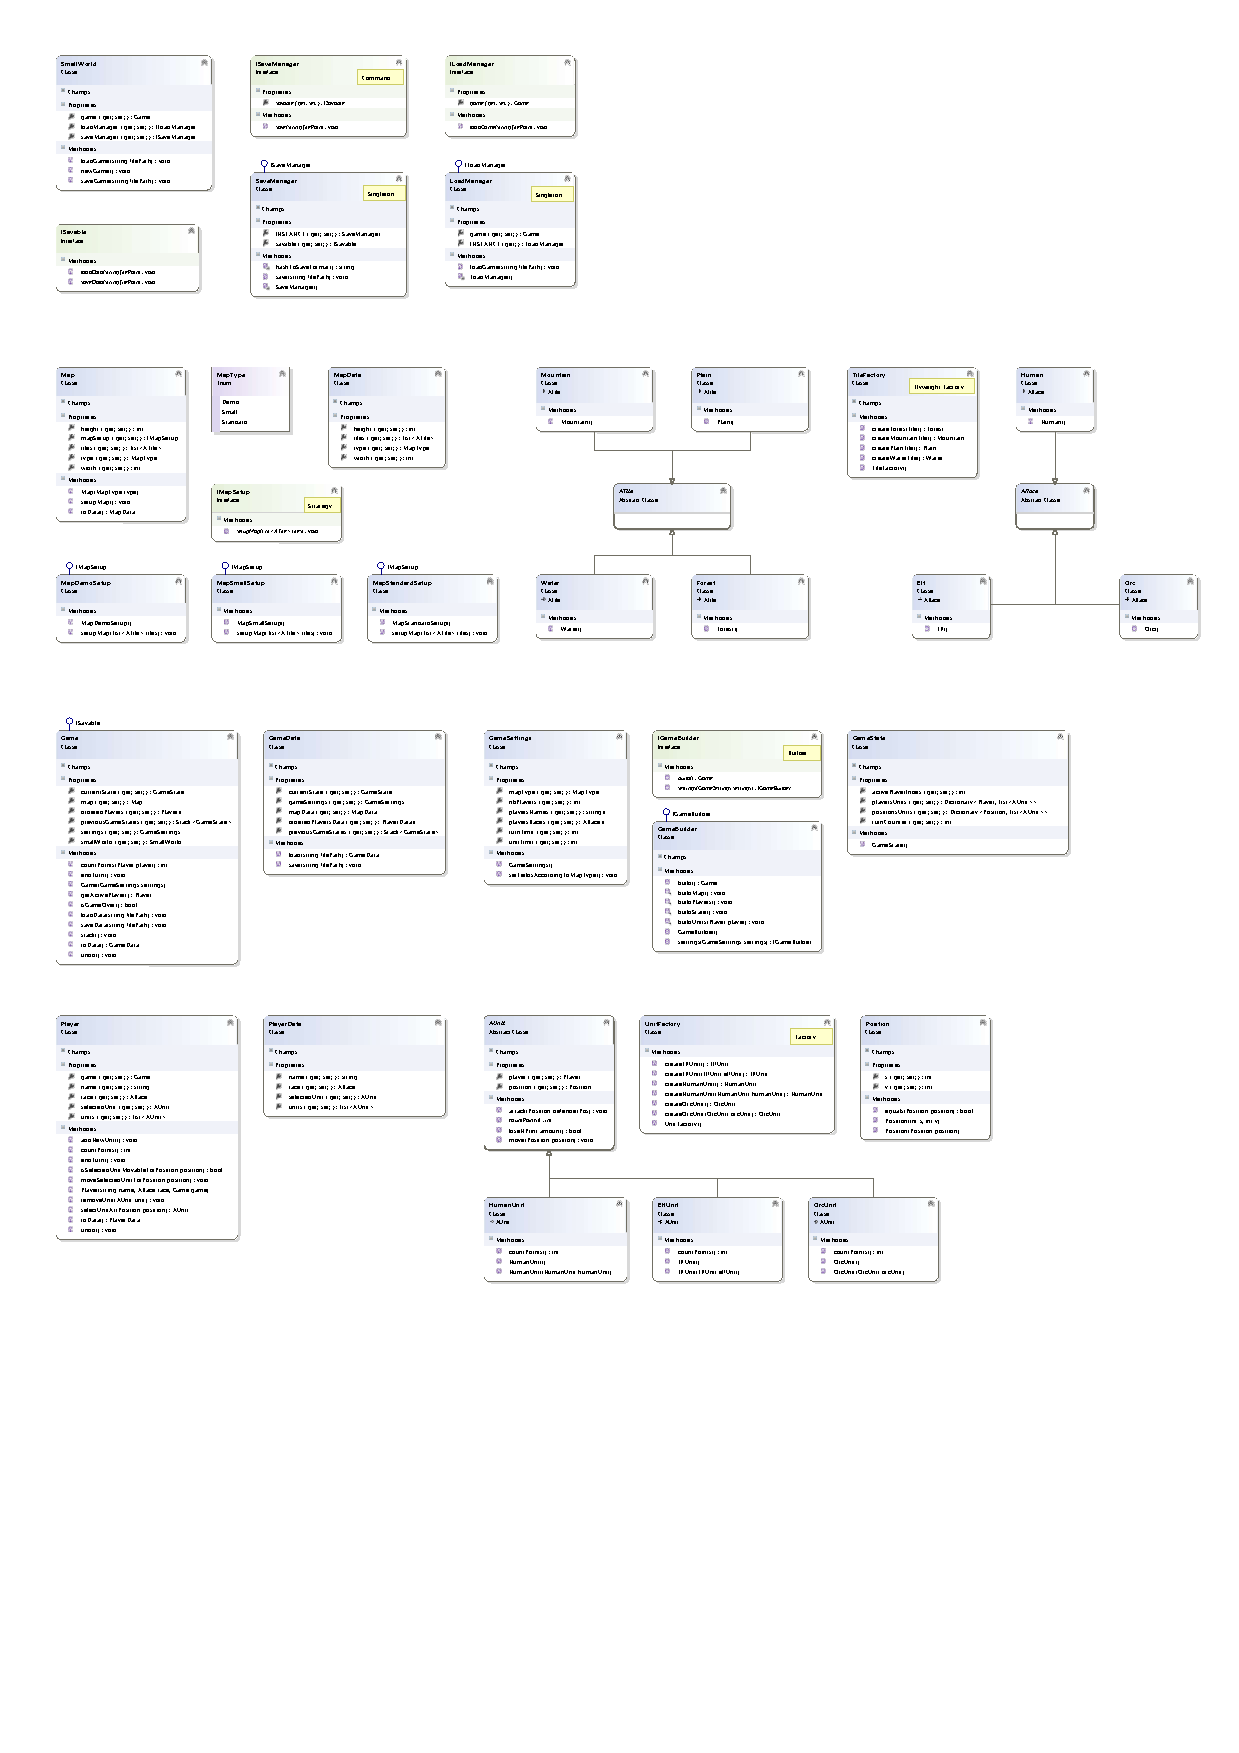
\includepdf{images/classDiagram.pdf}

\subsection{Diagrammes d'interaction}
\paragraph{}
Les diagrammes suivants permettent de détailler précisément les échanges entre les différentes instances de nos classes, dans deux traitements spécifiques.

\subsubsection{Diagramme de séquence : initialisation d'une partie}
Le diagramme suivant présente le processus d'initialisation d'une partie.

\paragraph{}
La partie est paramétrée par l'utilisateur au moyen de l'interface graphique. Ces informations sont ensuite regroupées dans un objet passé en paramètre de la création de la partie. La partie créé alors sa carte, et initialise son état courant.

\paragraph{}
Afin d'initialiser les objets joueurs, on répète les actions suivantes pour chaque joueur : 
\begin{itemize}
    \item Création d'une instance de joueur paramétrée par le nom et la race spécifiés (le joueur possède une référence vers la partie, et initialise son unité sélectionnée par défaut).
    \item Pour chaque unité affectée au joueur, on créé une unité de la race correspondante, et on l'ajoute à la liste des unités du joueur.
    \item On définit ensuite la position par défaut des unités du joueur.
    \item Ajout du joueur aux joueurs de la partie.
\end{itemize}

\paragraph{}
Une fois tous les joueurs initialisés, on tire au sort l'ordre de jeu, et on initialise la pile des états précédents.
La partie peut maintenant donner la main au premier joueur.

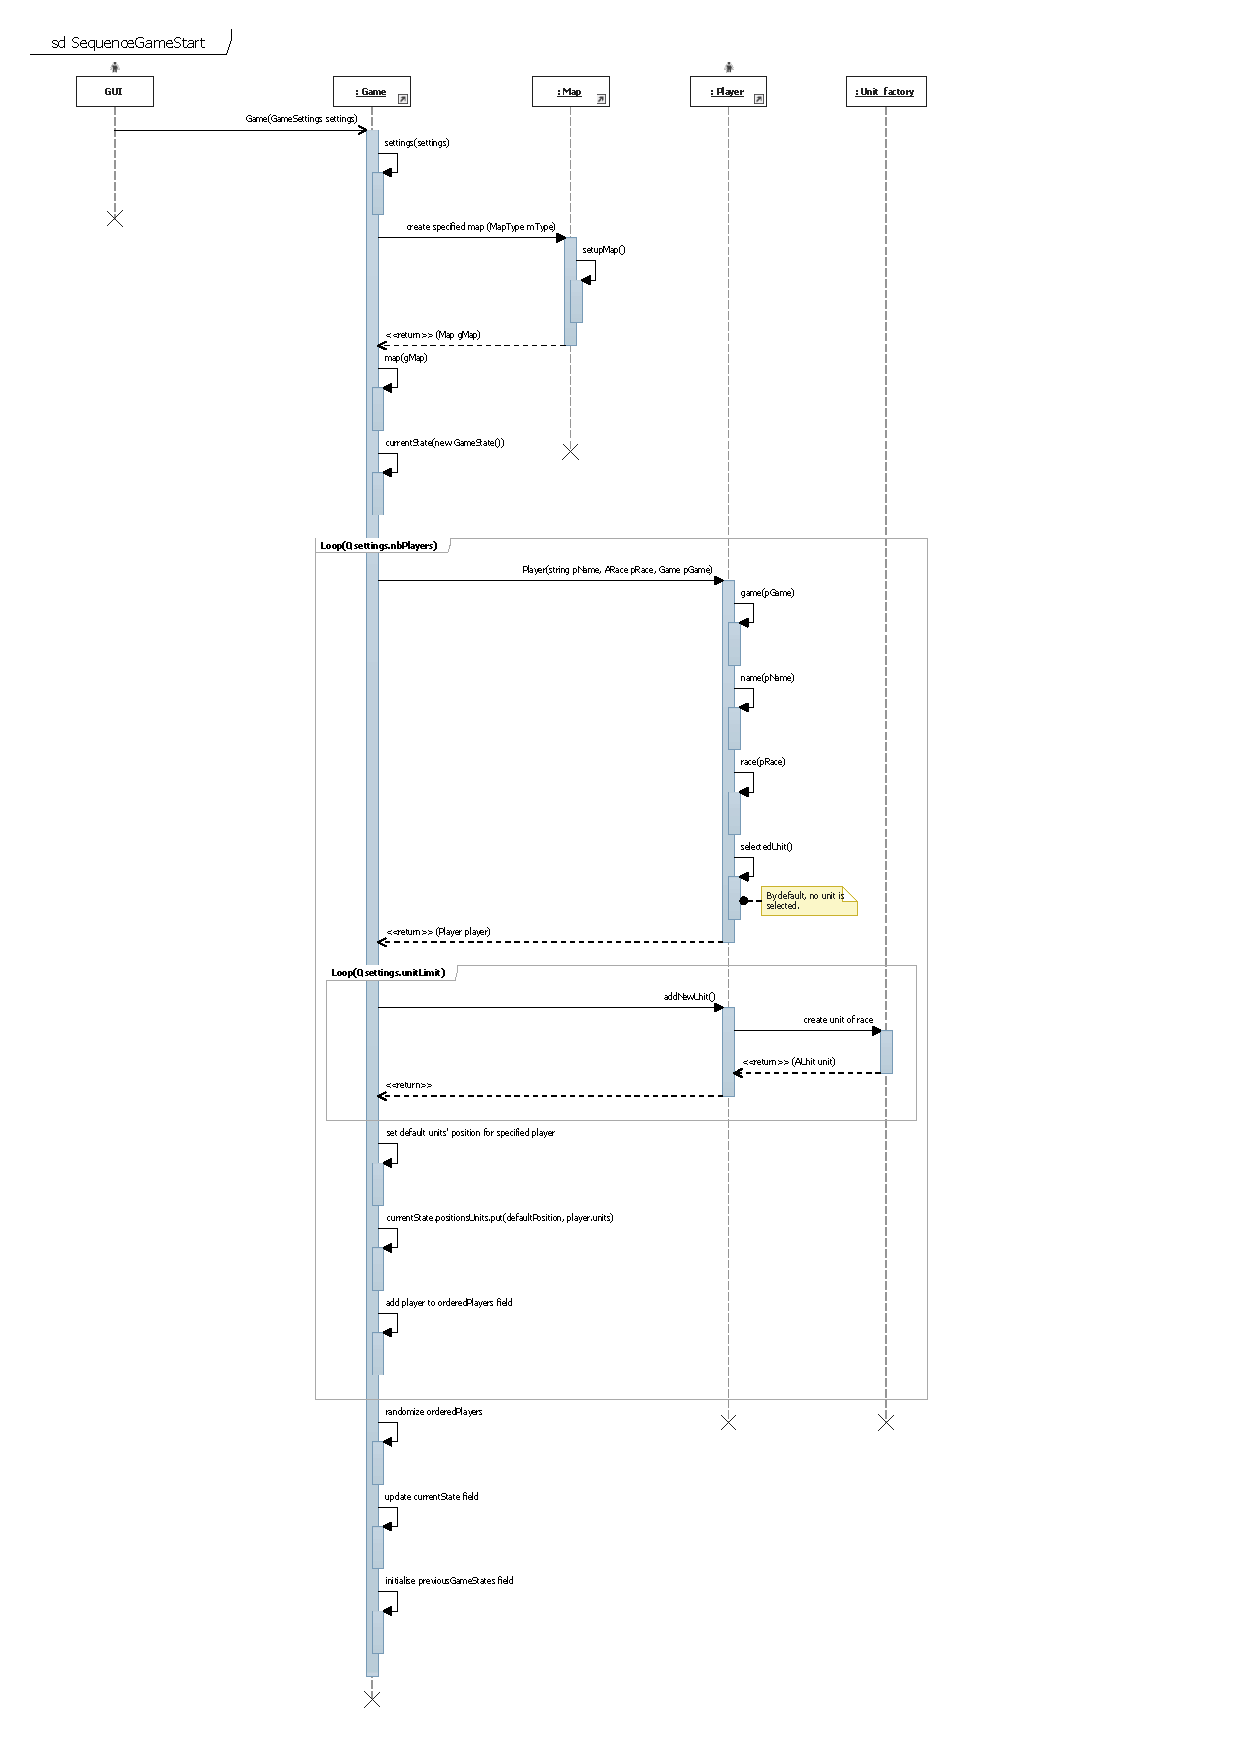
\includepdf{images/gameInitialisationSequenceDiagram.pdf}

\subsubsection{Diagramme de séquence : déroulement d'un tour}

Le diagramme suivant présente le déroulement d'un tour et aborde différentes actions typiques.

\paragraph{}
Au début du tour, le joueur courant \textit{sélectionne} une de ses unités. Il lui donne ensuite un ordre de \textit{déplacement}. Selon la case ciblée, on détermine la faisabilité du trajet. Si le trajet est impossible, rien ne se passe. Au contraire, si le trajet est possible, on détermine alors s'il s'agit d'un \textit{déplacement} (vers une case inoccupée ou occupée par des unités alliées), ou d'une \textit{attaque}. À la suite de quoi, le joueur informe la partie qu'un changement significatif va être effectué. Celle-ci enregistre alors l'état de jeu actuel, pour pouvoir y revenir si besoin.

\paragraph{}
Dans le cas d'un simple \textit{déplacement}, le joueur met à jour la position de l'unité sélectionnée, qui elle-même averti la partie des modifications qu'elle subit, afin que cette dernière mette à jour son état courant.

\paragraph{}
Dans le cas d'une \textit{attaque}, on effectue les traitements suivants :
\begin{itemize}
    \item Perte de points de vie de l'attaquant (en cas de décès de l'unité attaquant, on met à jour l'unité sélectionnée du joueur, et on supprime l'unité de sa liste d'unités, avant d'avertir la partie des nouvelles modifications).
    \item Perte de points de vie du défenseur (en cas de décès de l'unité du défenseur, on la supprime de la liste d'unités du joueur défenseur, avant d'avertir la partie des nouvelles modifications).
    \item Si le défenseur est mort, que l'attaquant a survécu, et qu'il n'y a plus de défenseurs sur la case ciblée, alors le joueur déplace l'unité attaquante jusqu'à la position spécifiée, avant d'avertir la partie des nouvelles modifications.
\end{itemize}

\paragraph{}
Dans les deux cas, le joueur peut répéter ces manipulations autant de fois qu'il le peut et le désire, avant de valider son tour. Il informe alors la partie de sa décision, qui va mettre à jour l'état courant, et les états précédents, afin de préparer le tour du joueur suivant.

\paragraph{}
Nous n'avons pas représenté ici les cas de victoire par élimination, ni spécifié le traitement du comptage des points à la fin du tour. De plus, le cas de l'utilisation de l'action \textit{undo} par le joueur n'a pas été traité. Le diagramme se concentre sur un tour typique, et non sur des cas exceptionnels. Bien entendu, tous ces cas seront traités dans le code, et nous les détaillons d'ailleurs dans la section \ref{DET}.

\paragraph{}
\textit{Remarque : }les traitements de perte de points de vie son conditionnés par le type des unités impliquées dans le combat (distance ou corps à corps). Ces considérations sont prises en compte dans la méthode de perte de points de vie.

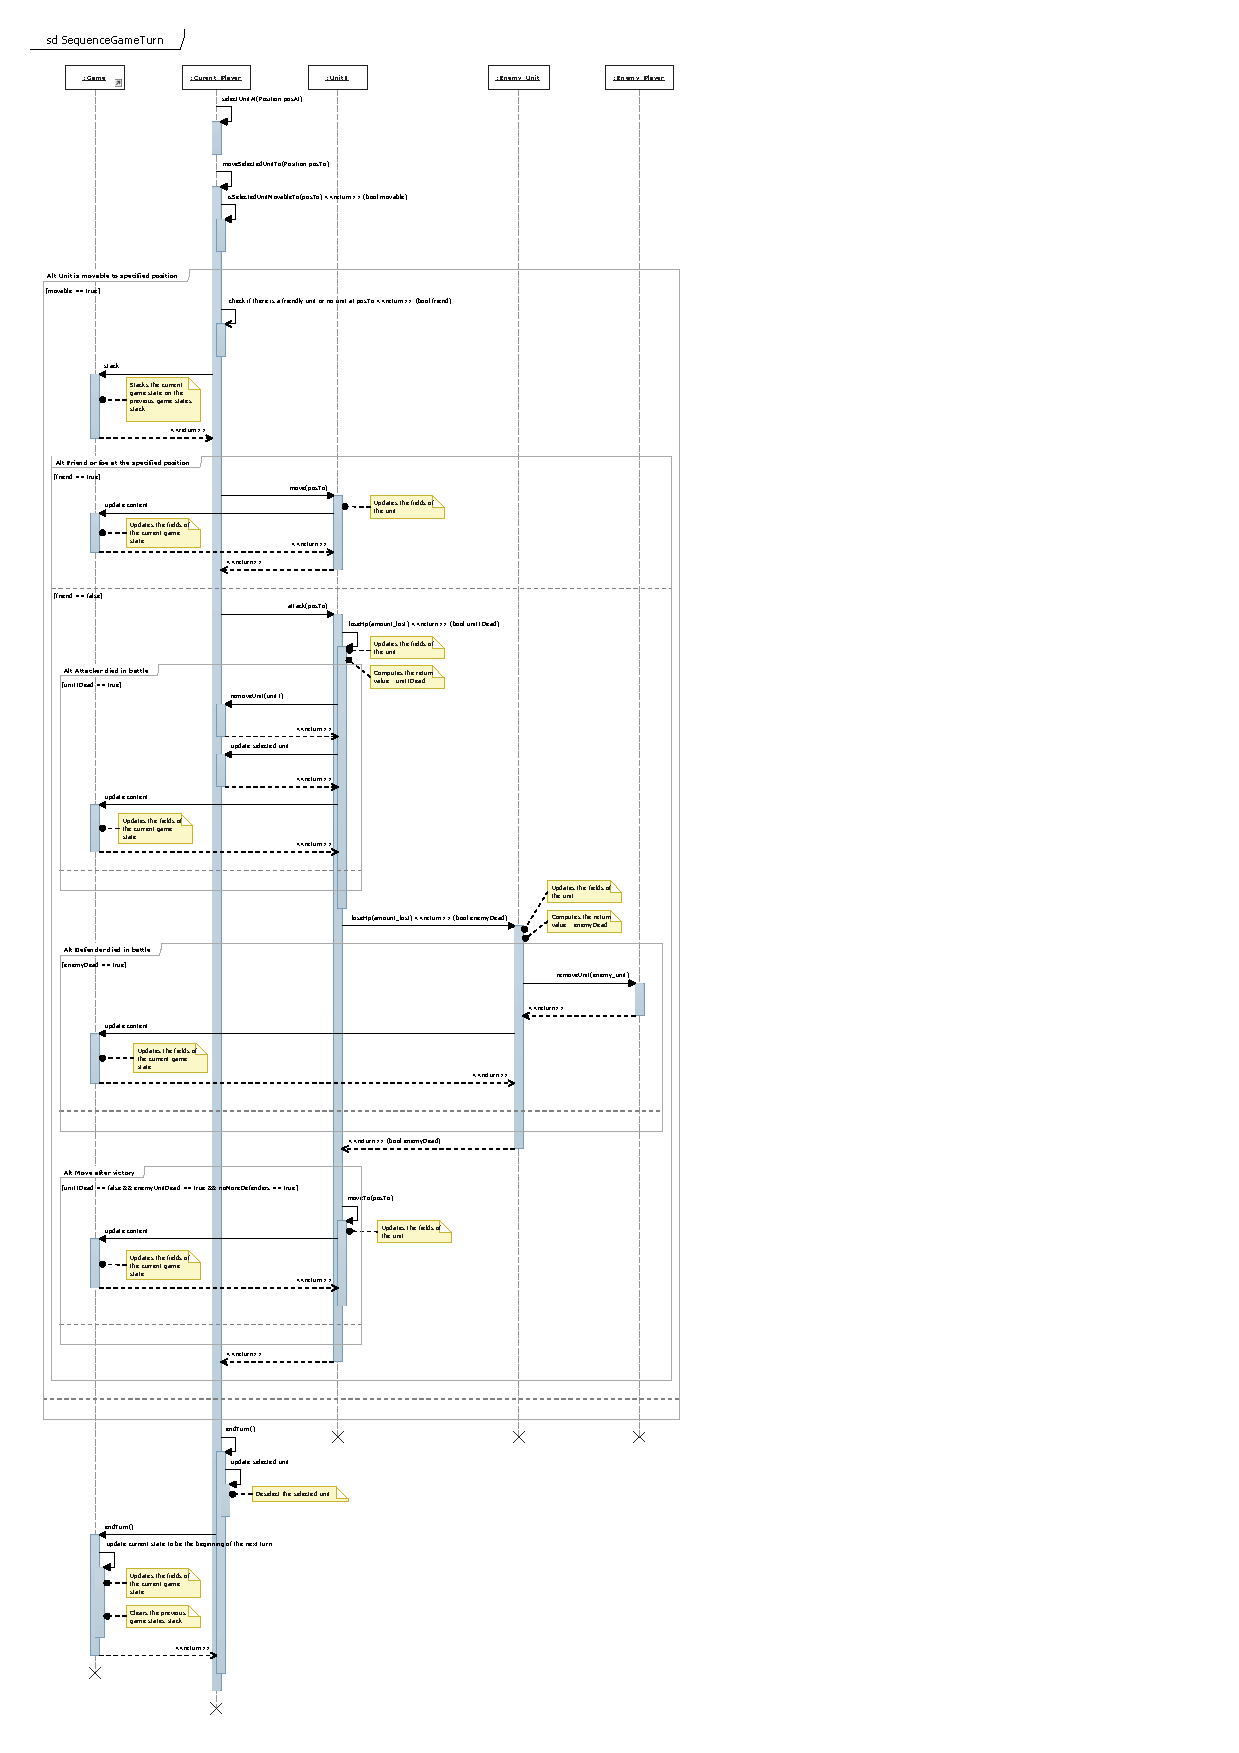
\includepdf{images/gameTurnSequenceDiagram.pdf}

\subsection{Diagramme d'états-transitions : états de la partie}
\label{DET}
Le diagramme suivant illustre les différents états d'une partie, et les évènements et conditions qui permettent une transition entre états.

\paragraph{}
En premier lieu, l'utilisateur détermine les paramètres de la partie (noms des joueurs, races, type de carte), puis ces informations sont transmises à la partie qui est alors \textit{paramétrée}. La partie s'\textit{initialise} alors selon les paramètres fournis. Durant cette phase, on détermine le joueur qui sera le premier à agir. La partie démarre alors un nouveau tour, et donne la main au premier joueur, que nous appellerons par la suite joueur 1.

\paragraph{}
Le changement de joueur s'effectue lors de l'annonce de fin de tour par le joueur 1. Si durant son tour, le joueur 1 est parvenu à éliminer toutes les unités de son adversaire, on arrive à la \textit{victoire du joueur 1}. Si le joueur 1 a perdu toutes ses unités durant son tour et décide tout de même de le valider, on arrive à la \textit{victoire du joueur 2}. Sinon, le jeu donne la main au joueur 2. De la même façon, on détermine si le joueur 2 gagne ou perd par élimination à la fin de son tour. On arrive alors à la \textit{fin du tour de jeu} (tous les joueurs ont eu leur tour). S'il reste des tours à jouer, la partie redonne la main au joueur 1.

\paragraph{}
À la fin du nombre limite de tours, si aucun des joueurs n'a atteint de victoire par élimination, on arrive à la \textit{fin de partie}. La partie détermine alors, en fonction des points de victoire accumulés par les deux joueurs, s'il s'agit d'une situation de \textit{victoire du joueur 1}, de \textit{victoire du joueur 2}, ou encore d'\textit{égalité}. La partie se termine alors.

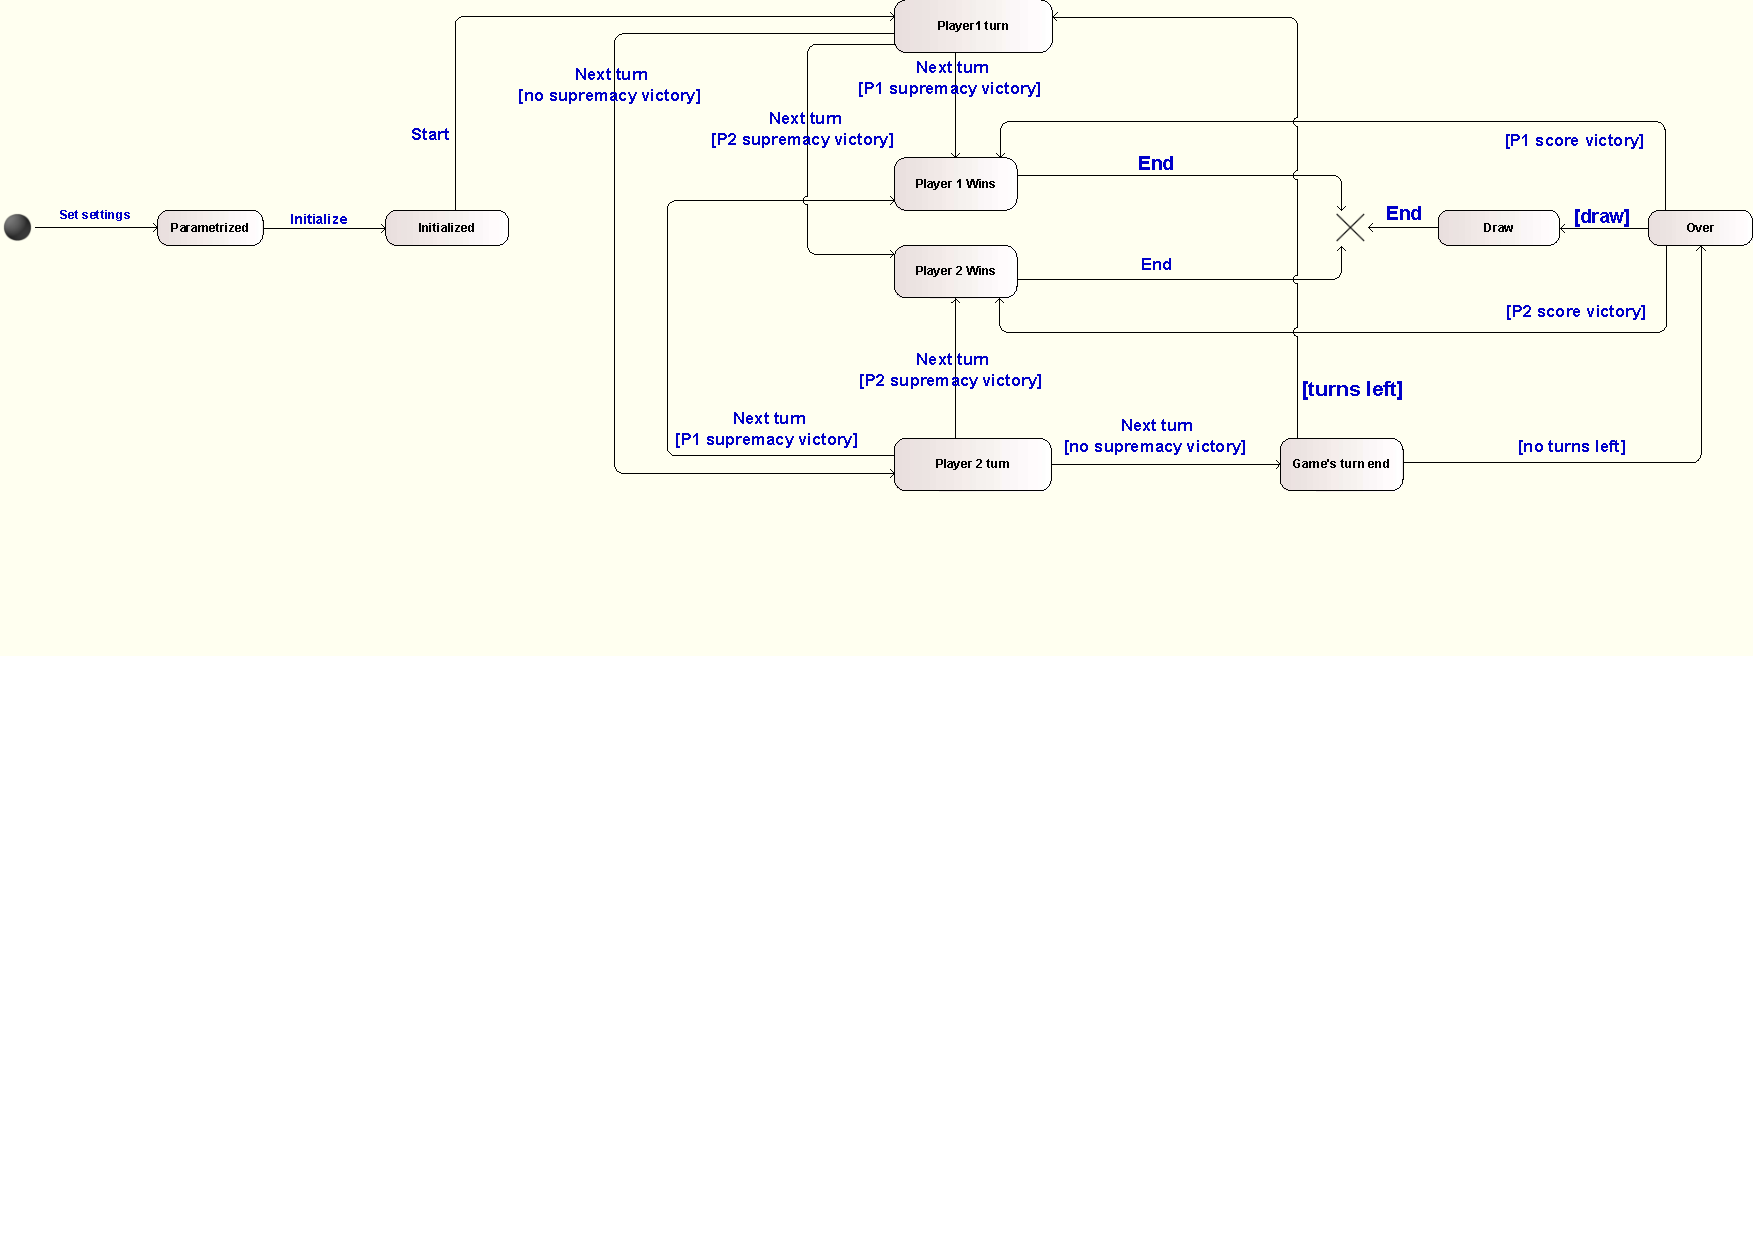
\includepdf[landscape=true]{images/gameStatechart.pdf}

\end{document}
